%% revmark_demo.tex  revmark.sty 的单页示例，内容虚构。
%% 编译  latexmk -xelatex -interaction=nonstopmode revmark_demo.tex   （需要两遍，图表内的批注依赖 TikZ overlay）
\documentclass[10pt]{article}
\usepackage[letterpaper,top=1in,bottom=1in,left=1.5in,right=1.5in]{geometry}
\usepackage{amsmath,booktabs,tikz}
\usepackage[colorlinks=true]{hyperref}
\usepackage{revmark}
\RevSetup{link color=2F3FAF}
%% reviewers.tex  审稿人编号与页边批注颜色的唯一来源。
%% 回复工程（rebuttal_main.tex）与修订稿（\usepackage{revmark} 之后）都读这个文件。
%% 格式 \RevReviewer{编号}{颜色 HTML}。编号写审稿系统给的编号，颜色避开修订红色。
\RevReviewer{R1}{7B3294}
\RevReviewer{R2}{00838F}
%% 示例色板依次是紫、青和棕色（5D4037），新增审稿人时继续取可与修订红和引用色区分的深色。

\setlength{\parskip}{4pt}

\begin{document}

\begin{center}
{\Large\bfseries OurSys: Budget-Constrained Duplicate Record Detection}\\[2pt]
{\small Anonymous authors}
\end{center}

\section{Selection under a labeling budget}
\label{sec:method}
OurSys chooses which candidate pairs to send for labeling under a fixed budget. Rule-based matchers such as R-Match score each pair in isolation~\cite{demo2024}.
\rev{The selection score of a candidate pair $p$ is the mean recall gain over the reference batches $B$, $s(p) = \frac{1}{|B|}\sum_{b \in B} \big(R(b \cup p) - R(b)\big)$, where $R$ is recall under the labeling budget.}{R1-W2}
A small edit of a few words stays in black and carries no note.

\section{Evaluation}
\label{sec:eval}
\rev{Each dataset now uses five data splits, and three training runs are averaged in each cell.}{R1-W1, R1-Q1}
\revred{This passage shares the note of its paragraph, so it is red without a second note.}
Section~\ref{sec:method} and Table~\ref{tab:main} keep the original wording, and the link colour marks them as references, as does the URL \url{https://example.org}.

\rev{At a budget of 2\% of the candidate pairs, OurSys reaches 0.799 against 0.763 for L-Boost.}{R2-W1}

\begin{table}[h]
\centering
\caption{\revcap{Recall at a budget of 5\% of the candidate pairs, mean over five data splits.}{R1-W1}}
\label{tab:main}
\begin{tabular}{lccc}
\toprule
Dataset & OurSys & L-Boost & L-Forest \\
\midrule
D1 & 0.880 & 0.840 & 0.816 \\
\revcap{D2}{R2-Q1} & \revred{0.831} & \revred{0.796} & \revred{0.782} \\
\bottomrule
\end{tabular}
\end{table}

\begin{figure}[h]
\centering
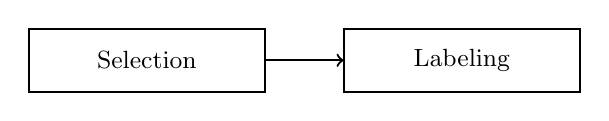
\begin{tikzpicture}
\draw[thick] (0,0) rectangle (3,0.8);
\node at (1.5,0.4) {\small Selection};
\draw[->, thick] (3,0.4) -- (4,0.4);
\draw[thick] (4,0) rectangle (7,0.8);
\node at (5.5,0.4) {\small Labeling};
\end{tikzpicture}
\caption{\revcap{Selection and labeling at the same budget.}{R2-Q1}}
\label{fig:flow}
\end{figure}

\begin{thebibliography}{1}
\bibitem{demo2024} A.~Author. A demonstration reference. 2024.
\end{thebibliography}

\end{document}
